\documentclass{article} % \documentclass{} is the first command in any LaTeX code.  It is used to define what kind of document you are creating such as an article or a book, and begins the document preamble

\usepackage{amsmath} % \usepackage is a command that allows you to add functionality to your LaTeX code
\usepackage{graphicx} % allows for images to be added to the latex document

\usepackage[T1]{fontenc}

\usepackage{hyperref} % allows for hyperlinks to be added to the document
\hypersetup{
    colorlinks,
    citecolor=black,
    filecolor=black,
    linkcolor=black,
    urlcolor=black,
    pdftitle={Research},
    pdfpagemode=FullScreen
}

\usepackage[
backend=biber,
style=numeric-comp,
sorting=ynt
]{biblatex} %Imports biblatex package
\addbibresource{references.bib} %Import the bibliography file

\graphicspath{{../pdf/}{./research_images}}

\title{Research} % Sets article title
\author{Sean Groenenboom \and Seger Sars \and Siem Vermeulen \and Angel Villanueva \and Ronan Vlak} % Sets authors name
\date{\today} % Sets date for date compiled
\newpage
\begin{document}

\maketitle % creates title using information in preamble (title, author, date)
\newpage

\tableofcontents % creates a table of contents
\newpage

\section{Seger}
\subsection{gamespeed}
How do game engines handle game speed?
\subsection{2d rendering}
How do game engines render 2d graphics?
\subsection{sprites}
How do game engines handle sprites?
\newpage
\section{Game speed}
Movement is a very important part of any game, but how is movement calculated accurately across different computers?
Different computers have different internals and thus run games with differing performance.
One computer might be able to run the games at 60FPS, but another can only run the game at 30FPS.
How can you make sure that both users have the exact same experience despite the difference in render speed.
A difference in render speed is shown in \autoref{fig:TimeBetweenFramesDisplayed} below.
\begin{figure}[h!]
    \centering
    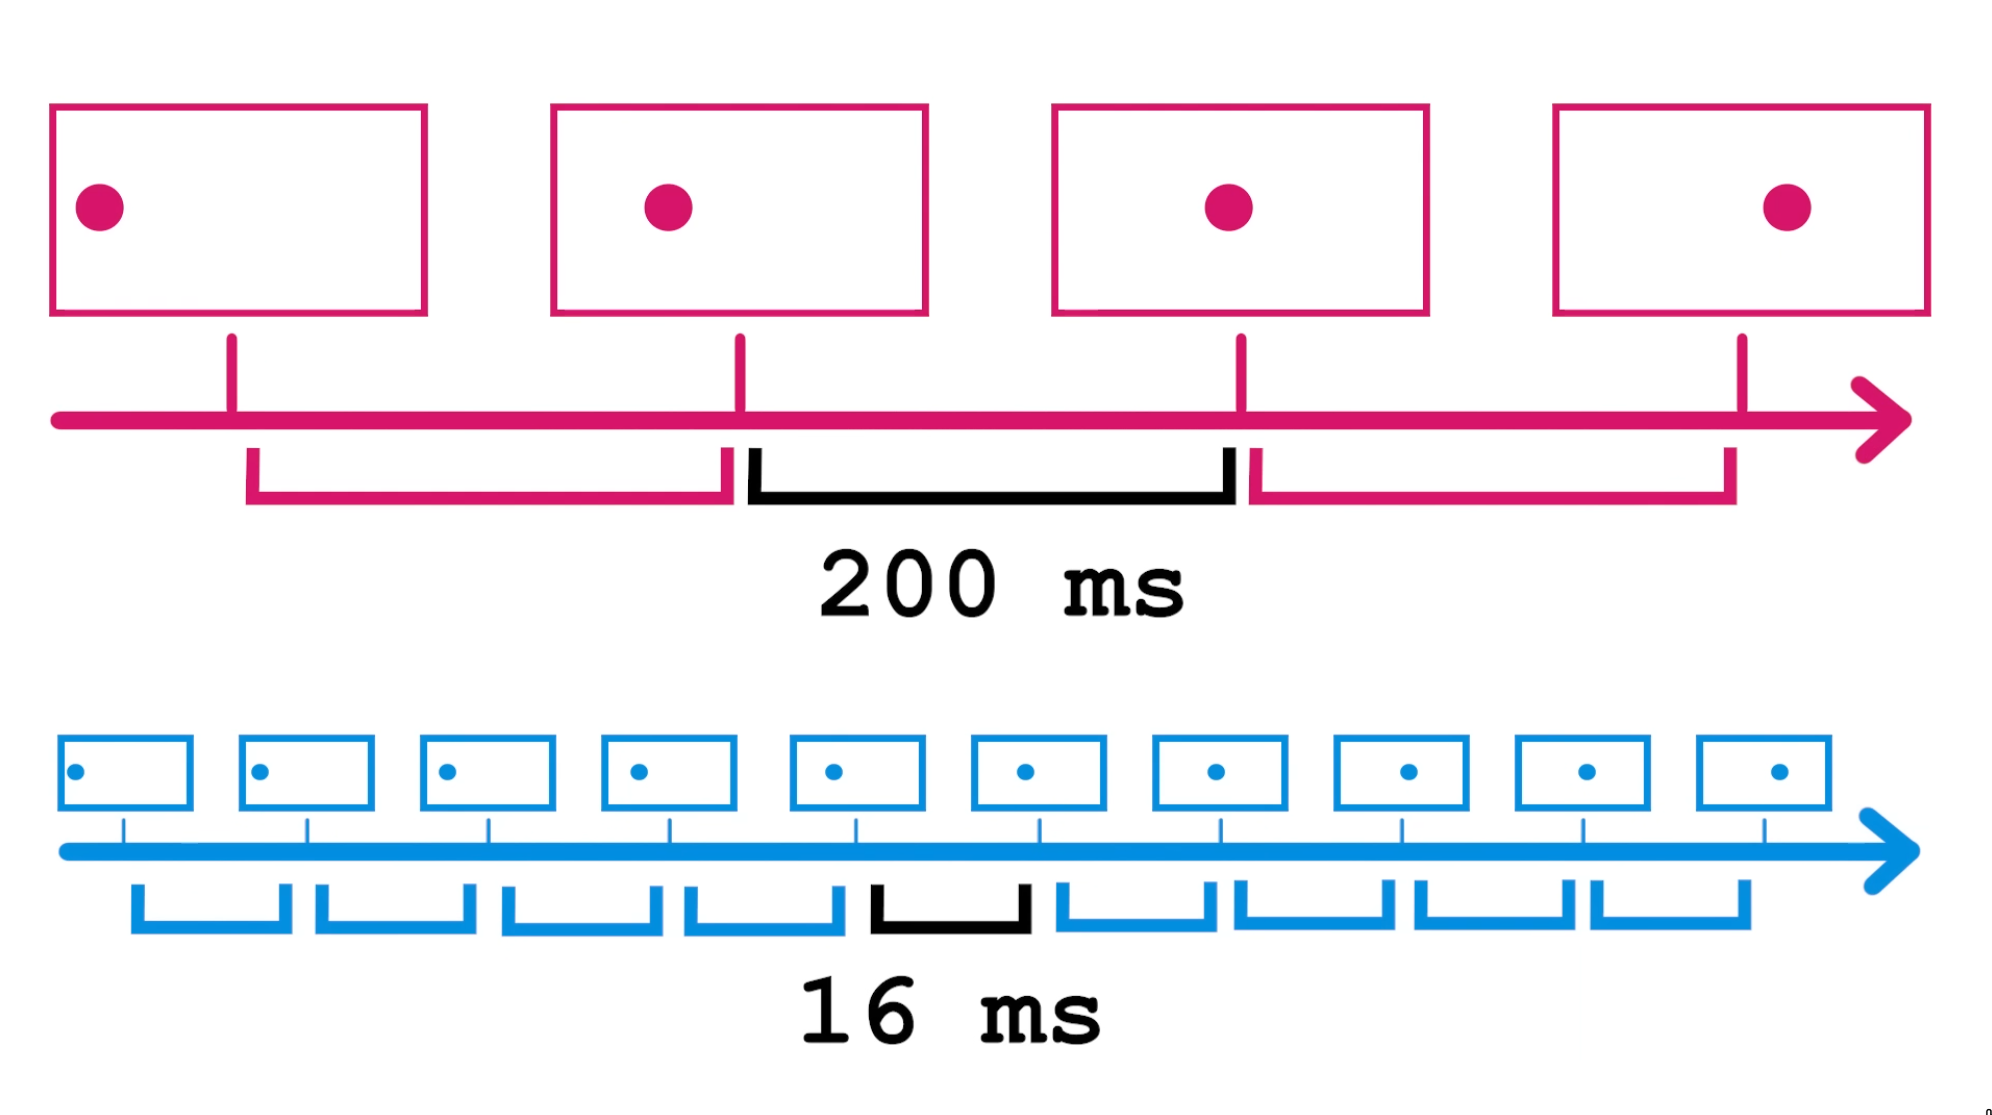
\includegraphics[width=0.8\textwidth]{time_between_frames.png}
    \caption{Time between frames displayed}
    \label{fig:TimeBetweenFramesDisplayed}
\end{figure}

\subsection{Potential problems}
A standard game loop runs one time each frame, before the frame is rendered.
The game loop is responsible for handling all the movement in the game, like moving the player.
If the game runs at 60FPS the game loop will be run 60 times each second.
\newline\newline
The following formula could be used to move the player each game loop iteration:
\newline
playerPosition.x = playerPosition.x + 10
\newline\newline
If this formula would be used to move the player, when running at 60PFS, the player would move 600 units of length each second.
But if the game was running at 30FPS, the player would only move 300 units each second.
So the player with 60FPS is considerably faster than the one with 30FPS.
This is of course, not ideal, as a game developer you want everyone to move at the same speed despite the computer it is run on.
The difference in elapsed distance is also shown in \autoref{fig:DifferenceInElapsedDistance} below.
\begin{figure}[h!]
    \centering
    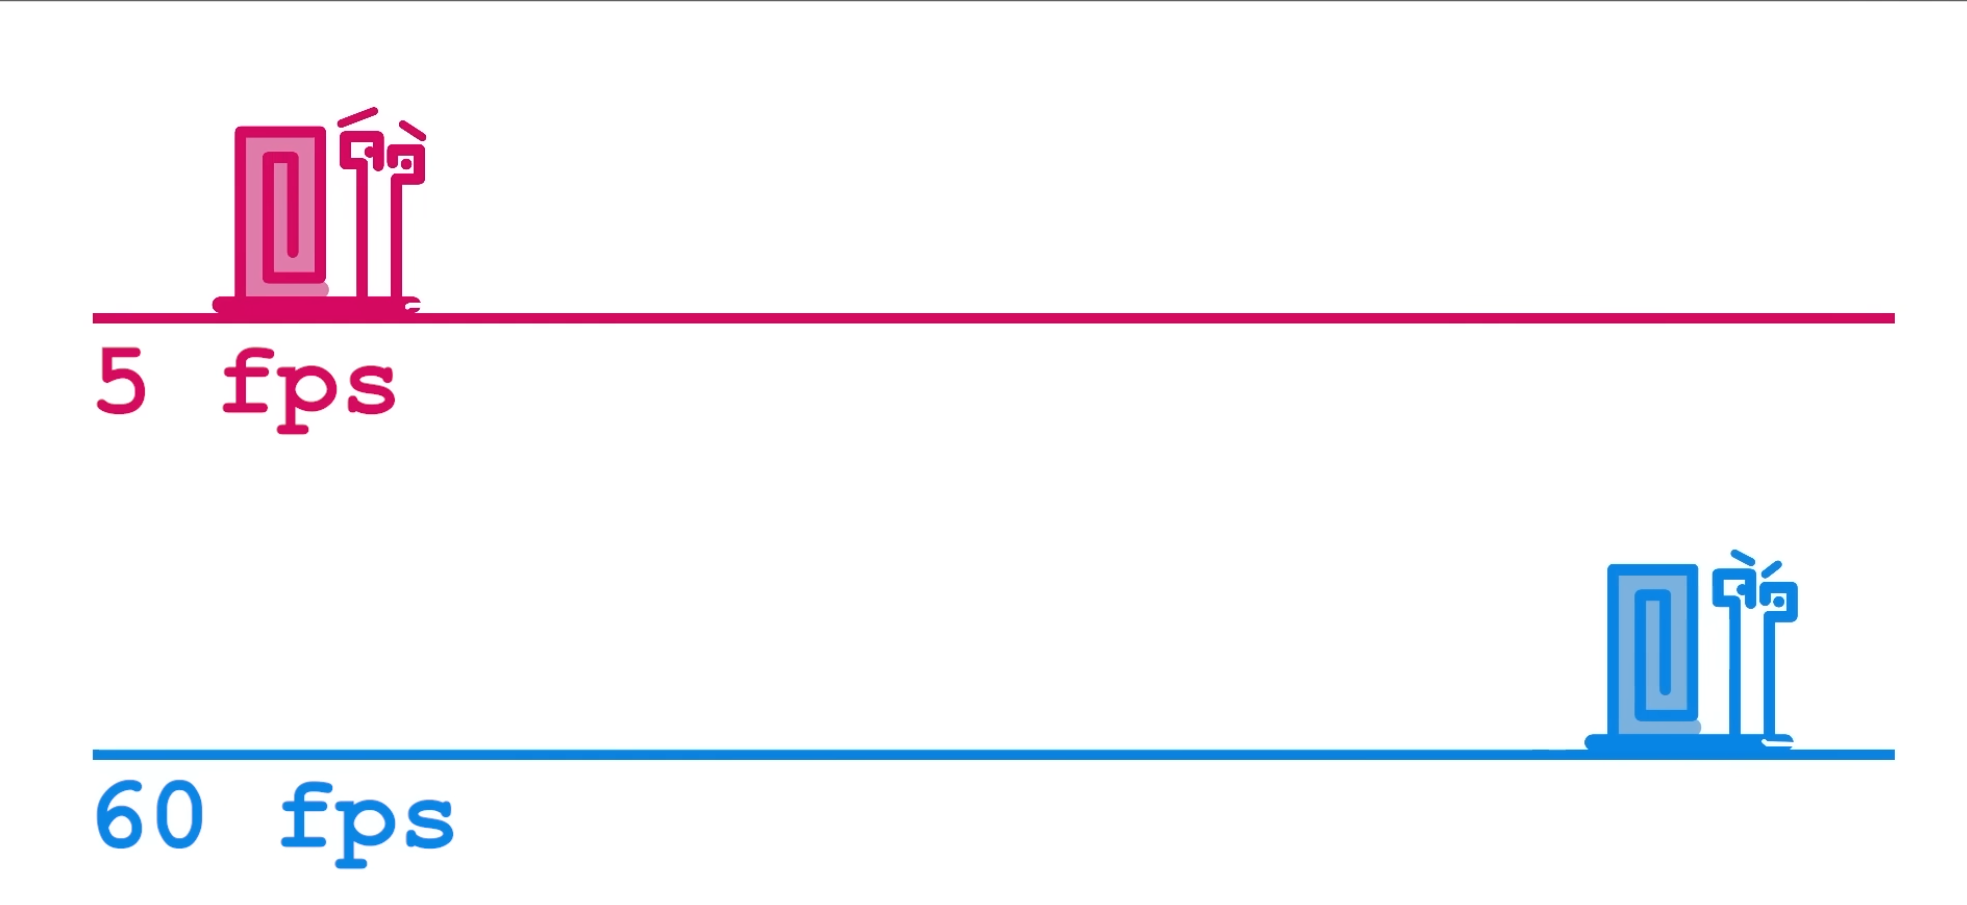
\includegraphics[width=0.8\textwidth]{difference_in_distance.png}
    \caption{Difference in elapsed distance}
    \label{fig:DifferenceInElapsedDistance}
\end{figure}

\subsection{Possible solutions}
There are two common solutions that help alleviate this problem, adjusting the movement speed relative to the FPS or making sure to handle movement in a fixed update loop that is guaranteed to run at a certain amount of cycles each second.

\subsubsection{Fixed update}
A solution to the differing movement speeds between computers, is to create a lightweight time based interrupt, often referred to as FixedUpdate, to handle all movement.
It is important that the FixedUpdate function is very small, otherwise the FixedUpdate could be too slow to be called at a constant rate each frame, defeating the purpose of the FixedUpdate.
In \autoref{fig:FixedUpdateView} below it is shown how times between different rendered frames can vary, while the FixedUpdate is called at a constant rate, where the small black bar represents the duration of the FixedUpdate function.
\begin{figure}[h!]
    \centering
    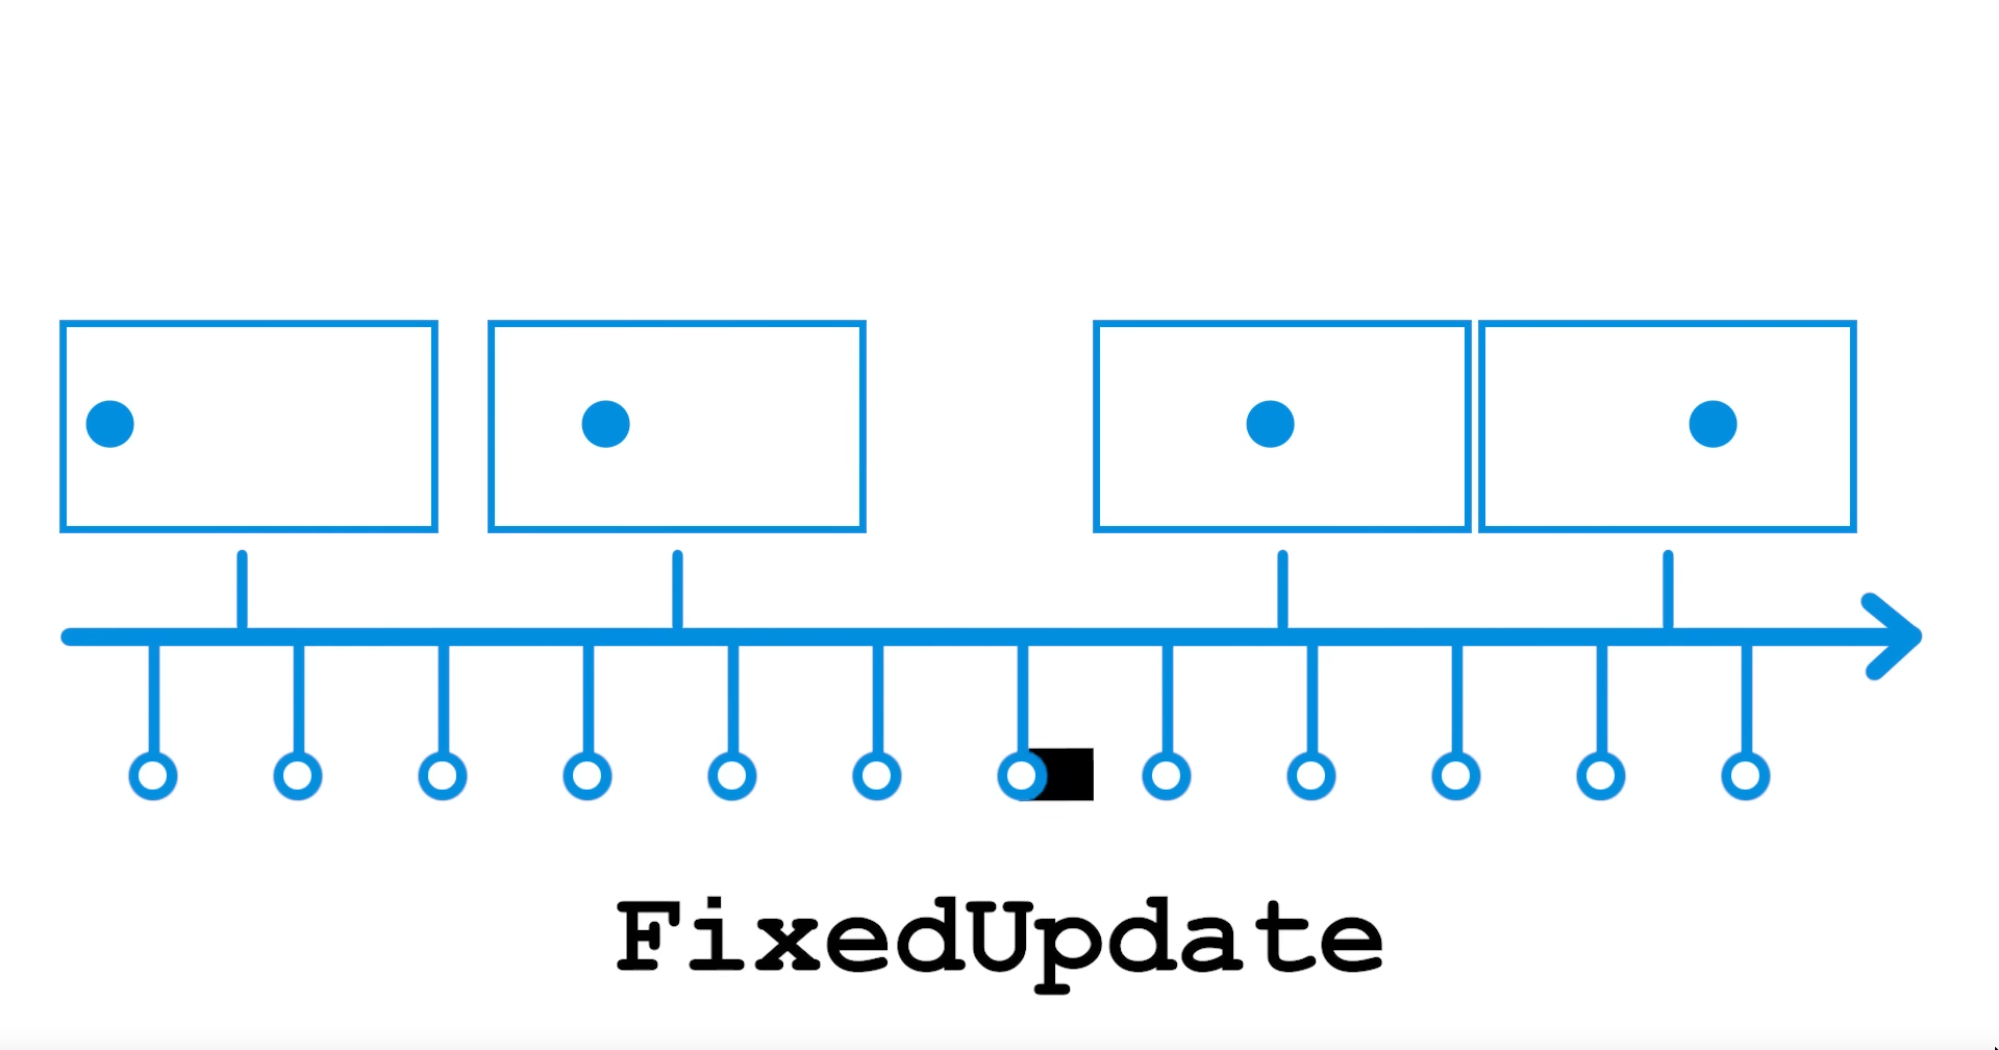
\includegraphics[width=0.6\textwidth]{fixed_update_explanation.png}
    \caption{Fixed update view}
    \label{fig:FixedUpdateView}
\end{figure}
\newline
If you were to use the same formula to calculate the player movement as before, it would now show constant movement between computers.

\subsubsection{Delta time}
Another solution to the differing speeds between computers, is to make the added distance when moving the player relative to the last time distance was added to the player.
Keeping track of every time movement is added to an object is not very efficient so this is solved in a slightly different manner.
So this means the formula would look like this:
\newline
playerPosition.x = playerPosition.x + (10 * deltaTime)
\newline
This uses the deltaTime variable to make the movement relative to the last time the movement was calculated.
\newline\newline
The deltaTime variable is calculated by the game engine and is globally accessible.
The game engine measures the time between the previous frame and the frame before, then assigns that value to the deltaTime variable.
This process is shown in \autoref{fig:DeltaTimeValueWhenUsingVariable}  below where the black square is the place deltaTime is used and the 0.14 is the time it took for the previous frame to render.
\begin{figure}[h!]
	\centering
	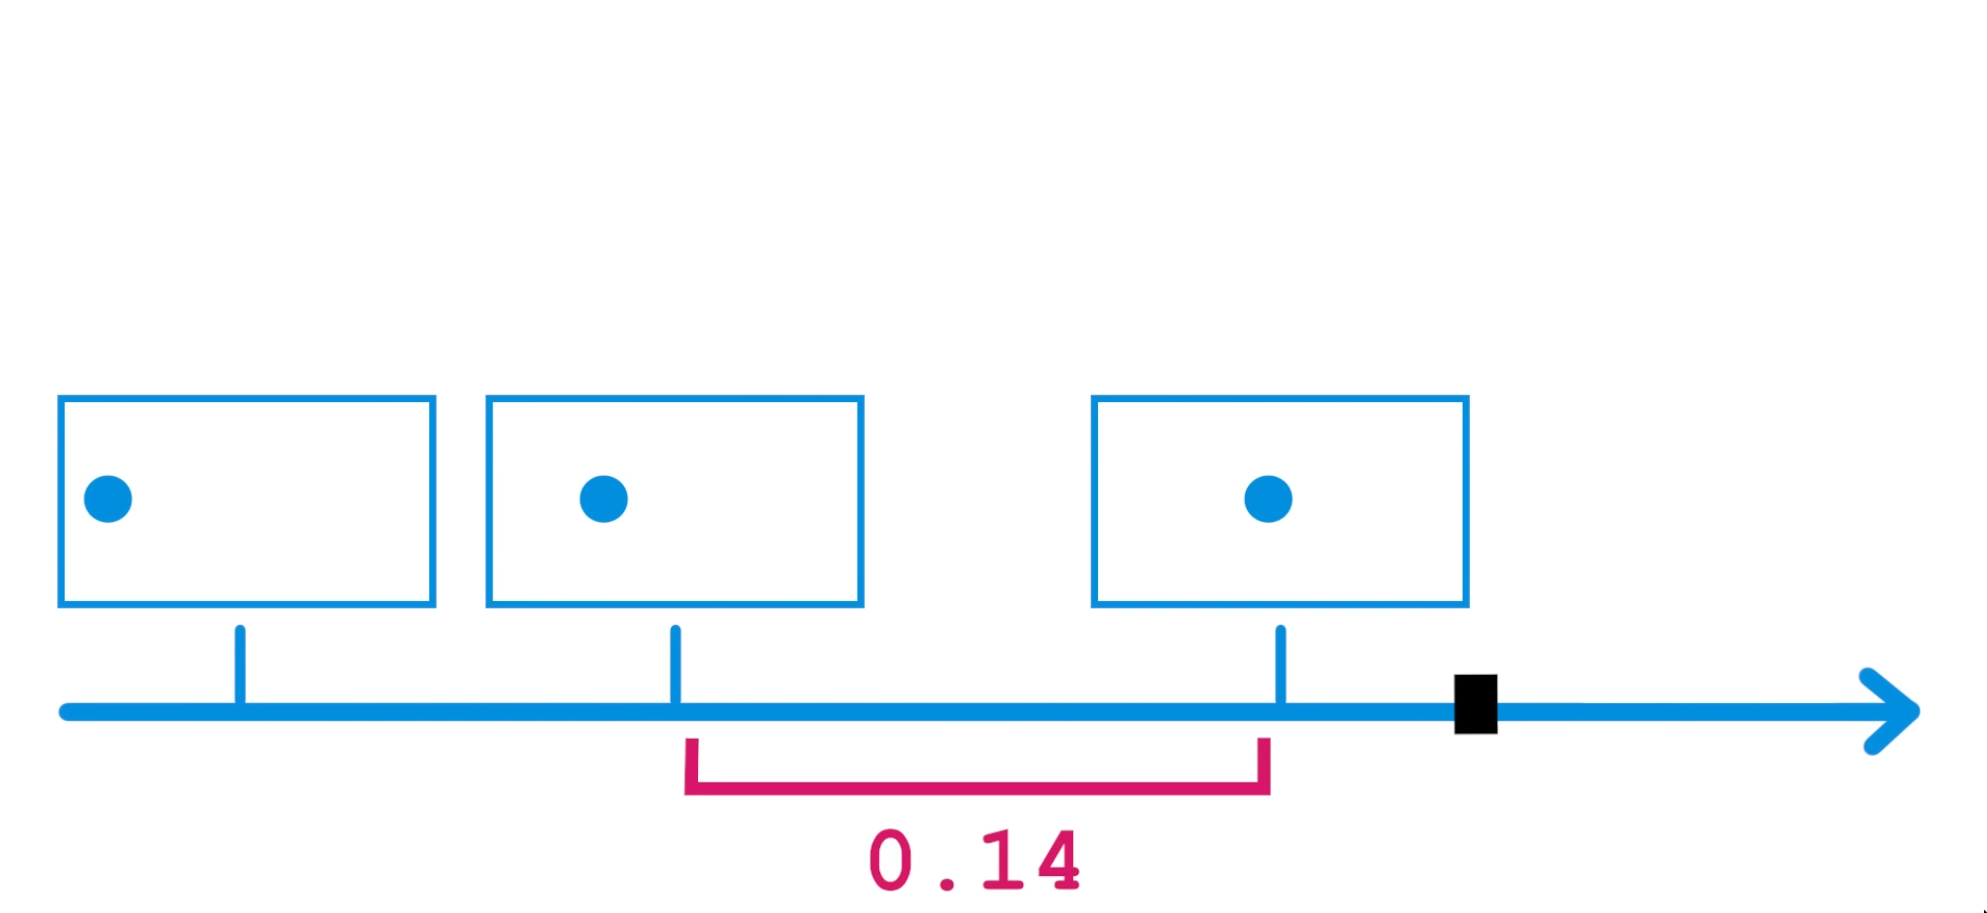
\includegraphics[width=0.6\textwidth]{used_deltatime_when_using_variable.png}
	\caption{deltaTime value when using variable}
	\label{fig:DeltaTimeValueWhenUsingVariable}
\end{figure}
\newline
Because deltaTime is used while rendering a frame, it is not possible to know how long it takes to render the rest of the frame.
This is why the value for the previous frame is used, although this means the deltaTime value lags behind by one frame, the delay is not noticable in most situations.

\newpage


\section{2D rendering}
The game engine has to be able to display and render images on screen.
The game engine will support 2D games, but how does the game engine render images to the screen?

\subsection{SDL2}
A simple way to get graphics working in you own custom application is to use a graphics library.
One of the most used simple 2D graphics libraries is SDL2.
SDL2 is a library written in C that allows the user to have very easy and lightweight cross-platform rendering capabilities.
SDL2 handles most things, so the user can start SDL2 and load and display images, without having to deal with the OS or GPU.
SDL2 does not only handle rendering images but is also capable of managing audio, keyboard, mouse and joystick, allowing for easy user input and audio management across different platforms.

\subsection{Cairo}
Like SDL2 Cairo offers a library written in C that allows the user to render text and images to the screen in a simple way.
Unlike SDL2 Cairo does not offer any access to sound, keyboar, mouse and joystick.
Cairo does not offer these features because the library is meant to be graphics only and as small as possible.

\section{raw doggen met OPENGL}
pijn
\newpage


\section{sean}
\subsection{Multiplayer}
Whhich are frequently used multiplayer structures?
\subsection{input}
How do game engines handle input?
controller
\subsection{ai}
What kind of ai do game engines usually have?
pathfinding?
\newpage

\section{Multiplayer}
Multiplayer is an important aspect of gaming. It is not necessary for a game to work, but it can greatly enhance the experience.
\subsection{Models}
There are multiple multipayer models each with their own advantages and disadvantages. \cite{Kroupp_2024}

\subsubsection{Client-Server Model}
The \textit{client-server} model is one of the most widely used architectures for multiplayer games. In this model, a server hosts the game world, and clients (players) connect to it. The server is considered authoritative, managing the game state and ensuring consistency across all clients.

\textbf{Advantages}
\begin{itemize}
    \item Ensures a consistent and authoritative game state.
    \item Reduces the risk of cheating, as the server controls the game logic.
    \item Scalable for large games (e.g., MMOs).
\end{itemize}

\textbf{Challenges}
\begin{itemize}
    \item Requires a reliable and performant server, which adds complexity and cost.
    \item Introduces latency between clients and the server, which can affect gameplay responsiveness.
\end{itemize}

\subsubsection{Peer-to-Peer (P2P) Model}
In the \textit{peer-to-peer} model, all players (peers) are directly connected to each other, and the game state is shared among them. Each peer has equal authority over the game, which can make synchronization and consistency more difficult to maintain.

\textbf{Advantages}
\begin{itemize}
    \item Simple to implement for small-scale games with a limited number of players.
    \item No need for a dedicated server, reducing costs.
\end{itemize}

\textbf{Challenges}
\begin{itemize}
    \item Difficult to ensure game state consistency across peers.
    \item Susceptible to cheating, as each peer has authority.
    \item Latency and synchronization issues are harder to manage.
\end{itemize}

\subsubsection{Authoritative Server with Client-Side Prediction}
This model combines the \textit{client-server} approach with \textit{client-side prediction}. The server remains authoritative, but clients predict the outcome of their actions while awaiting confirmation from the server. This reduces the apparent latency for the player.

\textbf{Advantages}
\begin{itemize}
    \item Provides a smoother and more responsive experience for players.
    \item Retains the security and consistency of a server-authoritative system.
\end{itemize}

\textbf{Challenges}
\begin{itemize}
    \item Complex to implement, requiring careful handling of discrepancies between predicted and actual outcomes.
    \item Still subject to latency, although mitigated by prediction.
\end{itemize}

\subsubsection{State Synchronization}
In \textit{state synchronization}, the server periodically sends the full game state to clients, ensuring that all players have a consistent view of the game world.

\textbf{Advantages}
\begin{itemize}
    \item Simple to implement for games where maintaining a consistent game state is critical, such as strategy or turn-based games.
    \item Ensures that all clients are synchronized with the server.
\end{itemize}

\textbf{Challenges}
\begin{itemize}
    \item Can be bandwidth-intensive, especially for games with a large or complex game state.
    \item Latency can lead to noticeable delays in the game state being updated on clients.
\end{itemize}

\subsubsection{Event-Driven Networking}
\textit{Event-driven networking} focuses on sending specific events (e.g., player actions) rather than the entire game state. Clients process these events and update their local game state accordingly.

\textbf{Advantages}
\begin{itemize}
    \item More efficient in terms of bandwidth, as only small packets of information are transmitted.
    \item Suitable for games with frequent, small state changes, such as mobile or social games.
\end{itemize}

\textbf{Challenges}
\begin{itemize}
    \item Requires careful ordering and processing of events to ensure consistency.
    \item Can be difficult to implement for games with complex interactions.
\end{itemize}

\subsubsection{Hybrid Models}
Many games use a \textit{hybrid} approach, combining aspects of different multiplayer models to optimize performance, scalability, and security. For example, a game might use the client-server model for general game logic but implement peer-to-peer connections for specific tasks like voice chat or trading.

\textbf{Advantages}
\begin{itemize}
    \item Offers flexibility to tailor the multiplayer system to different aspects of the game.
    \item Allows for optimization of performance and scalability where needed.
\end{itemize}

\textbf{Challenges}
\begin{itemize}
    \item Increases complexity, requiring careful design to ensure all components work seamlessly together.
    \item May require more effort to maintain and debug.
\end{itemize}

\subsection{Tools}
The development of multiplayer games requires specialized tools and frameworks to ensure smooth,
real-time communication between players, game servers, and clients. Whether it's managing the networking stack, handling player synchronization, or reducing latency,
choosing the right multiplayer tool is crucial to the success of any game. This chapter explores the most commonly used multiplayer tools for professional game developers,
followed by a section specifically aimed at student developers using C++.

\subsubsection{Commonly Used Multiplayer Tools for Professional Developers}
Professional game developers often need multiplayer tools that are scalable, feature-rich, and easy to integrate with large, complex projects. The tools listed below are widely used in the industry for various types of multiplayer games.

\paragraph{Unity} (with Netcode for GameObjects or Mirror)
is one of the most popular game engines for both 2D and 3D game development,
and it provides several options for multiplayer networking.
\\
\textbf{Advantages}:
\begin{itemize}
    \item Extensive documentation and community support.
    \item Tight integration with Unity's development workflow.
    \item Multiple networking solutions, including Netcode for GameObjects (official) and Mirror (open-source).
\end{itemize}
\textbf{Disadvantages}:
\begin{itemize}
    \item Limited scalability for very large multiplayer projects.
    \item Mirror, while simple, may require additional setup for complex use cases.
\end{itemize}

\paragraph{Unreal Engine} (with Unreal Networking) Unreal Engine,
a high-end game engine used in AAA titles, includes built-in support for multiplayer via its advanced networking framework.
\\
\textbf{Advantages}:
\begin{itemize}
    \item Built-in support for replication and remote procedure calls (RPCs).
    \item Highly scalable, suitable for large multiplayer games.
    \item Excellent graphics and physics, suitable for visually intensive games.
\end{itemize}
\textbf{Disadvantages}:
\begin{itemize}
    \item Steep learning curve, especially for new developers.
    \item Resource-intensive, requiring powerful hardware for development.
\end{itemize}

\paragraph{Photon Engine} is a cloud-based multiplayer framework designed to scale from small indie games to large multiplayer experiences.
\\
\textbf{Advantages}:
\begin{itemize}
    \item Cloud-hosted and scalable.
    \item Supports both authoritative server and peer-to-peer networking models.
    \item Easy integration with Unity and Unreal Engine.
\end{itemize}
\textbf{Disadvantages}:
\begin{itemize}
    \item Requires a Photon cloud subscription for larger projects.
    \item May add latency depending on the geographical location of servers.
\end{itemize}

\paragraph{Godot} (with ENet or Nakama) Godot is a free,
open-source game engine that supports both 2D and 3D games.
It has a lightweight networking stack using libraries such as ENet or Nakama.
\\
\textbf{Advantages}:
\begin{itemize}
    \item Free and open-source, ideal for indie developers.
    \item Lightweight and fast, especially for 2D games.
    \item Community-driven development and support.
\end{itemize}
\textbf{Disadvantages}:
\begin{itemize}
    \item Lacks the advanced tools found in Unity or Unreal for larger games.
    \item Smaller community compared to other engines.
\end{itemize}

\paragraph{PlayFab} is a backend service for multiplayer games that provides tools like player authentication, leaderboards, and matchmaking.
\\
\textbf{Advantages}:
\begin{itemize}
    \item Fully managed backend service, reducing server-side complexity.
    \item Integrates with multiple game engines.
    \item Scales for small and large games.
\end{itemize}
\textbf{Disadvantages}:
\begin{itemize}
    \item Requires an active subscription for large-scale use.
    \item May not offer the same level of control as self-hosted solutions.
\end{itemize}

\subsubsection{Multiplayer Tools for C++ Student Developers}
For student developers working with C++,
multiplayer tools must be lightweight, flexible, and simple to integrate.
Below are some commonly used tools for networking in C++ game projects.

\paragraph{ENet} is a reliable UDP-based networking library designed for real-time multiplayer games.
\\
\textbf{Advantages}:
\begin{itemize}
    \item Lightweight and easy to integrate.
    \item Provides reliable UDP, packet sequencing, and fragmentation.
    \item Perfect for real-time, fast-paced multiplayer games.
\end{itemize}
\textbf{Disadvantages}:
\begin{itemize}
    \item Does not offer high-level features such as matchmaking or player authentication.
    \item Requires manual implementation of game-specific features like lag compensation.
\end{itemize}

\paragraph{RakNet} (or SLikeNet) is a feature-rich networking engine designed for multiplayer games. SLikeNet is its actively maintained fork.
\\
\textbf{Advantages}:
\begin{itemize}
    \item Supports advanced features such as NAT punch-through, RPCs, and object replication.
    \item Cross-platform, with easy integration into various game engines.
    \item Highly suitable for both small and large multiplayer games.
\end{itemize}
\textbf{Disadvantages}:
\begin{itemize}
    \item More complex to learn and use compared to simpler libraries like ENet.
    \item RakNet’s development has slowed, although SLikeNet remains maintained.
\end{itemize}

\paragraph{asio} (Boost.Asio or standalone) is a general-purpose C++ networking library that supports both TCP and UDP communication and focuses on asynchronous I/O.
\\
\textbf{Advantages}:
\begin{itemize}
    \item Powerful and flexible, allowing developers to build custom networking solutions.
    \item Works well for both small-scale and large-scale projects.
    \item Supports asynchronous programming, which is crucial for multiplayer games.
\end{itemize}
\textbf{Disadvantages}:
\begin{itemize}
    \item Low-level, so developers need to implement most game-specific networking logic.
    \item Steeper learning curve due to its focus on concurrency and asynchronous programming.
\end{itemize}

\paragraph{KCP} (A Fast and Reliable UDP Protocol) KCP is a reliable and efficient UDP-based protocol for low-latency multiplayer games.
\\
\textbf{Advantages}:
\begin{itemize}
    \item High-performance, optimized for low-latency environments.
    \item Easy to integrate with existing networking systems.
\end{itemize}
\textbf{Disadvantages}:
\begin{itemize}
    \item Lacks higher-level features such as matchmaking, lobbies, or session management.
    \item Requires developers to implement their own game logic on top of the protocol.
\end{itemize}

\paragraph{Steamworks SDK} is a set of tools and services provided by Valve for games that are distributed via the Steam platform. It provides networking solutions as well as other features such as achievements, leaderboards, and user authentication.
\\
\textbf{Advantages}:
\begin{itemize}
    \item \textbf{Integration with Steam}: Provides seamless integration with the Steam platform, including achievements, leaderboards, and Steam Cloud.
    \item \textbf{Peer-to-peer and server-based networking}: Supports both peer-to-peer connections and server-authoritative networking models.
    \item \textbf{Matchmaking and lobbies}: Built-in support for lobbies, matchmaking, and friend invites, making it easier to manage multiplayer game sessions.
\end{itemize}

\textbf{Disadvantages}:
\begin{itemize}
    \item \textbf{Limited to Steam}: Only useful for games distributed via Steam, limiting its use for cross-platform or non-Steam games.
    \item \textbf{Requires Steam API knowledge}: Developers need to be familiar with Steam's API, which adds complexity to the development process.
\end{itemize}

\newpage

\section{Audio}
Sound can be considered to be an unmissable part of any video game. It is therefore important for any video game engine to 
support audio playback, and optionally to play multiple audio sources simultaneously and to give these audio sources a sense of physical direction.
\subsection{Audio on Linux}
Firstly, the following question must be answered: how is audio played on Linux through C++? The answer to this question can be divided into two types:
playing audio by directly interfacing with the operating system, or using third-party software to manage the audio playback.
Because of the lack of sources on the former, only the latter is considered in this research.

There are many audio libraries available for C++ on Linux, some of the most popular of which (intended for usafe in video games) are \cite{Szanto_2018}:
\begin{itemize}
    \item FMOD
    \item IrrKlang
    \item OpenAL
    \item SDL2 \footnote{SDL 2 is "a cross-platform development library designed to provide low level access to audio" \cite{sdl2}. It is therefore not strictly designed for just audio playback, but it is extensively used across the industry \cite{sdl2games}.}
\end{itemize}

\subsubsection{FMOD} is a proprietary \footnote{Its tools are free for teams with a revenue of < \$200.000 \cite{fmodStudio}.} sound engine used (mainly) in video games.
It is "widely used within the gaming industry", and "is globally regarded as the leading tools for the creation and playback of interactive audio" \cite{dolbyFmod}.

FMOD provides four different products:
\begin{enumerate}
    \item FMOD Studio: the software used to create and adding sound and music to a game. In-game, these sounds are played using the FMOD Engine \cite{fmodStudio}.
    \item FMOD for Unity: similar to FMOD Studio, but integrated into the Unity engine \cite{fmodUnity}.
    \item FMOD Core: a more low-level alternative to FMOD Studio. As opposed to FMOD Studio, which has a GUI, Core is only available through an API \cite{fmodCore}.
    \item FMOD.io: a library of various sound effects / files \cite{fmodIo}.
\end{enumerate}


\subsection{Multiple audio sources}
How can multiple sounds be played simultaneously?
\subsection{Directional audio}
How can stereo headphones be used to create directional audio?
\section{save data}
What are common save data structures?
encryptie? 
\newpage

\section{angel}
\section{particles}

Jeff Lander coins the term "Fuzzy" as a way of describing a type of object which lacks well-defined surfaces such as smoke or fire. \cite{Lander_1998} These objects contain a set of characteristics which makes it difficult to model as an object due to its random and chaotic nature. To solve this problem game engines make use of particle systems to generate particles/objects in a chaotic and controlled environment to recreate these effects.

\subsection{What is a particle system}

Compared to regular objects, Particle systems create objects which undergo a complete lifecycle. Within the life cycle, particles are created, change direction or properties, and dissappear again. Through the use of parameters controlling properties such as direction and duration a particle can appear random and natural while still following a set of determined rules to follow.

\subsection{Examples of particle systems}



What are particles in games?
What are common methods game engines use to render particles?

\newpage

\section{Physics}

Physics within games are a key component when it comes to creating realism between the interaction of objects and their physical properties such as velocity, density etc. 

\subsection{The use of physics engines}

Within video games, physics engines make use of mathematical algorithms and models to realistically calculate the physical behaviour of objects within a game \cite{Ipacs_2023}. The data produced by these engines can then be used to animate objects and detect collision between objects. This method saves time and creates more realism when animating objects.

\subsection{Examples of physics engines}

\subsubsection{Box2D}

Box2D is currently one of the most popular 2D physics libraries on github and describes itself as a "2D rigid body simulation library for games" \cite{Catto_2024}.

\subsubsection{LiquidFun}

LiquidFun is an expansion on the previously mentioned Box2D (reference to previous section). It contains the original features of Box2D but expands on it by adding "particle based fluid and soft body simulation" \cite{Miles_2014}.

\subsubsection{Chipmunk2D}

Chipmunk2D aims to provide "a simple, lightweight, fast and portable 2D rigid body physics library" \cite{Slembcke_2023}.

\newpage

\section{Levels (Ronan)}
\subsection{Levels in videogames}
A level in a videogame is a space available to a player during 
the completion of an objective. Levels are designed to present a challenge, 
objective, or puzzle that players must overcome to advance. 
There are a few aspects that might make up a level in a videogame:
\begin{itemize}
	\item Progression
	\item Design/Environment
	\item Objectives
	\item Difficulty
	\item Possible story advancement
\end{itemize}

\subsection{Level transitions}
Level transitions allow a player from level to another.
Level transitions can be one or two way.
A two way level transition can be used so a player can travel back and forth between connected levels.
One way level transitions prevent players from the traveling back to previous levels.
There a few common ways to manage the transition between levels:
\begin {itemize}
	\item
\end{itemize}
\subsection{Scenes}
\subsection{Storing levels}
\subsection{Third party level editors}

\section{Game objects (Ronan)}
\subsection{Game objects in a game engines}
\subsection{Adding components to game objects}

\newpage

\section{temp}
bullet hell engine
\\
2d engine.
\\
wow factor: veel entiteiten op het scherm. gamepseed ver kunnen verogen.
performance tot de max.
\\
seger:
gamespeed
2d rendering
sprites (animatie + matrix berkeningen(rotere, schalen etc))
\\
sean:
Multiplayer
hoe connecten naar elkaar (ip adres, username?)
wie host? Central? peer to peer?
\\
input + controller support
ai
\\
siem:\\
audio + adaptive music\\
data opslaan (voortgang, levels, statistieken, unlocks, achievements, etc)\\
\\
angel:\\
particles?\\
physics\\
\\
ronan:\\
levels + levels switchen + scenes + hud \\
gameobject
\\

example of a reference \cite{Gambetta_2024} like this test.


\newpage

\section{Annex}
\printbibliography %Prints bibliography

\end{document} % This is the end of the document
